\documentclass[10pt]{article}
\usepackage{geometry}                
\geometry{a4paper}
\usepackage{graphicx}
\usepackage{amssymb}
\usepackage{amsmath}
\usepackage{paralist}
\usepackage[parfill]{parskip}
\usepackage{float}
\usepackage{capt-of}


\title{TMA4215 Numerical Mathematics: Project 2 \\ Replace this line with your own title} 
\author{Student nr. 6XXXXX and 7XXXXX} % Here you insert the student number of the members of the group.
\date{\today}

                                          
\begin{document}
\maketitle
\begin{abstract}
This paper takes on piecewise curve-fitting with cubic Bezier curves, and an algorithm for this is presented. The method minimizes the number of curves used in the fitting. Two test problems of different character are included to show the performance of our algorithm.
\end{abstract}

\section*{Introduction} 
We have used Newton-Raphson iteration to find an optimal parametrization for the curve-fitting. \cite{Plass:1983} gives a method for this, and how to find values for the initial parametrization such that the iteration converges. We present a method of how to split the curve for an efficient algorithm for piecewise approximation. The algorithm returns the control points and the number of segments for the resulting curve generated by our method, and is further extended to making smooth shapes without sharp edges.


\section*{Theory and Method}

\subsection*{Bezier curves and Bernstein polynomials}

We have used cubic Bezier curves to approximate a given curve $\gamma$. From \cite{wiki:Bezier} and  we have that Bezier curves are parametrized curves consisting of sums of Bernstein polynomials:
\begin{align}
B_{i}^n(t) = \binom{n}{i}t^i(t-1)^{(n-i)},\quad i = 0, 1, ..., 0,\quad t \; \in \; [0,1].
\end{align}
A Bezier curve of degree n is given by
\begin{align}
\mathbf{S}(t) = \sum_{i=0}^{n} \mathbf{P}_i B_{i}^n(t), \quad 0 \leq t \leq 1,
\end{align}
where $\mathbf{P}_i$ are so called control points, chosen such that $\mathbf{P}_0$ and $\mathbf{P}_n$ are interpolation points between the Bezier curve and $\gamma$.


\subsection*{Finding control points}

For the best fit, $\mathbf{P}_1$ and $\mathbf{P}_2$ have to be chosen such that the distance between $\gamma$ and our Bezier curve is small. That is, we needed to minimize the the following expression:

\begin{equation}
E = \frac{1}{m} \sum_{i=1}^{m} \| \mathbf{x}_i - \mathbf{S}(t_i)\|^2_2,
\end{equation}

for parametrization values $t_i \in [ 0,1 ]$ and points $\mathbf{x}_i$ on $\gamma$. To do this we use a property of the Bezier curves: The two straight lines between $\mathbf{P}_0$ and $\mathbf{P}_1$, and $\mathbf{P}_2$ and $\mathbf{P}_3$ are tangents to the curve at $\mathbf{P}_0$ and $\mathbf{P}_3$ respectively:

\begin{align}
\mathbf{P}_1 = \mathbf{P}_2 + \alpha_1 \mathbf{v}_0 \\
\mathbf{P}_2 = \mathbf{P}_2 + \alpha_2 \mathbf{v}_3,
\end{align}

where $\mathbf{v}_0$ and $\mathbf{v}_3$ are unit tangent vectors of $\gamma$ at the endpoints. Since $\mathbf{P}_0$ and $\mathbf{P}_3$ are known from the points on the curve $\gamma$, this problem is reduced to finding $\alpha_1$ and $\alpha_2$ such that $E$ is small. To find where $E$ is smallest, we differentiate $E$ with respect to $\alpha_1$ and $\alpha_2$ and set the expressions to equal zero. To ease the reader we omit the whole process, and only state the resulting system of equations for $\alpha_1$ and $\alpha_2$:


\begin{align}
\alpha_1 \sum_{i = 1}^m B_1(t_i)^2 |\mathbf{v}_0|^2 + \alpha_2 \sum_{i = 1}^m B_1(t_i)B_2(t_i)\mathbf{v}_0 \cdot \mathbf{v}_3 
= - \sum_{i = 0}^m B_1(t_i) \mathbf{v}_0 \cdot \mathbf{A}_i, \\
\alpha_1 \sum_{i = 1}^m B_1(t_i)B_2(t_i)\mathbf{v}_0 \cdot \mathbf{v}_3 + \alpha_2 \sum_{i = 1}^m B_2(t_i)^2 |\mathbf{v}_3|^2 
= - \sum_{i = 0}^m B_2(t_i)\mathbf{v}_3 \cdot \mathbf{A}_i,
\end{align}

where $\mathbf{A}_i = \mathbf{P}_0(B_0(t_i) + B_1(t_i) + \mathbf{P}_3(B_3(t_i) + B_2(t_i)) - \mathbf{x}_i$.





\subsection*{Choosing initial $t$-values and Newton-Raphson Iteration}

To find the parametrization giving the smallest distance between the Bezier curve and $\gamma$, we differentiate the distance between the two curves with respect to $t$ and equate to 0:

\begin{align}
f(t) =  2(X(t)-x)X'(t) + 2(Y(t)-y)Y'(t) = 0.
\end{align}

Here, $X(t)$ and $Y(t)$ are coordinates on the Bezier curve, and $x$ and $y$ are coordinates on $\gamma$. This is a fifth-degree equation for $t$, and we use the Newton-Raphson iterative method,

\begin{align}
t \gets t - \frac{f(t)}{f'(t)},
\end{align}

to find the solution. This method will converge for the right starting values for $t$. We use initial $t$-values given by the distance between the data points, $x$ and $y$, from the curve $\gamma$. This method is merely based on \cite{Plass:1983}. Let

\begin{equation}
s_k = \sum_{i=1}^{k-1} \sqrt{(x_{i+1}-x_i)^2 + (y_{i+1}-y_i)^2}
\end{equation}

be the length of the polygonal segment from 1 to $k$, $k$ = 1, 2, ..., $n$. The initial parametric value is then $t_k = s_k/s_n$.

As seen from Figure~\ref{fig:Newton-Raphson}, this method converges quickly, so few steps are required for a $t$-value close enough to the root. We can see how the $t$-values in Figure \ref{fig:Newton-Raphson} are quite shifted after 3 iterations, from the green lines to the red lines. It is important that the values are still in range 0 to 1, so this needs to be checked after the iterations. 

\begin{figure}[H]
\centering
\begin{minipage}[t]{.43\textwidth}
\vspace{0pt}
    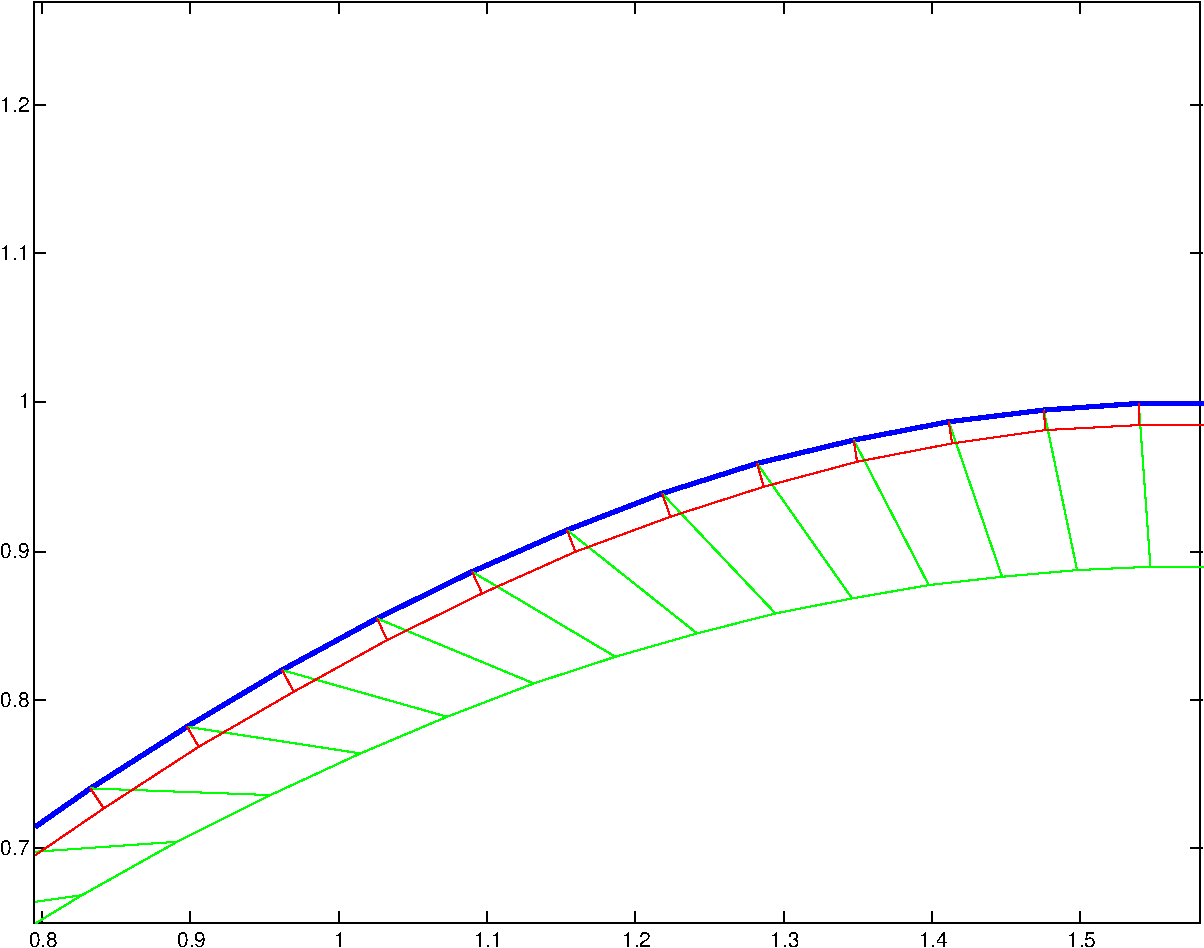
\includegraphics[scale=0.41, clip=true, trim = 0 0 0.9cm 5.5cm]{newtons3-crop.pdf}
\end{minipage}\hfill
\begin{minipage}[t]{.4\textwidth}
\vspace{0pt}
\captionof{figure}{Result after 3 Newton-Raphson iterations. The blue curve ($\gamma$) is a part of a sine function. The green curve is the Bezier curve with initial $t$-values. The red curve is the Bezier curve after 3 iterations. A straight line represents the distance between a point on $\gamma$ and the corresponding point on the Bezier curve.}
\end{minipage}
\label{fig:Newton-Raphson}
\end{figure}


\subsection*{Dividing the curve in two}
After using Newton-Raphson, if the error between $\gamma$ and the Bezier curve is still above the tolerance, it is possible to divide the curve in two. This can be done simply by choosing the point, $\mathbf{P}_i$, where the error is largest. Figure~\ref{fig:kurvedeling1} and Figure~\ref{fig:kurvedeling2} show how this splitting is done on an example curve. 


\begin{figure}
\centering
\begin{minipage}[t]{.45\textwidth}
\centering
\vspace{0pt}
    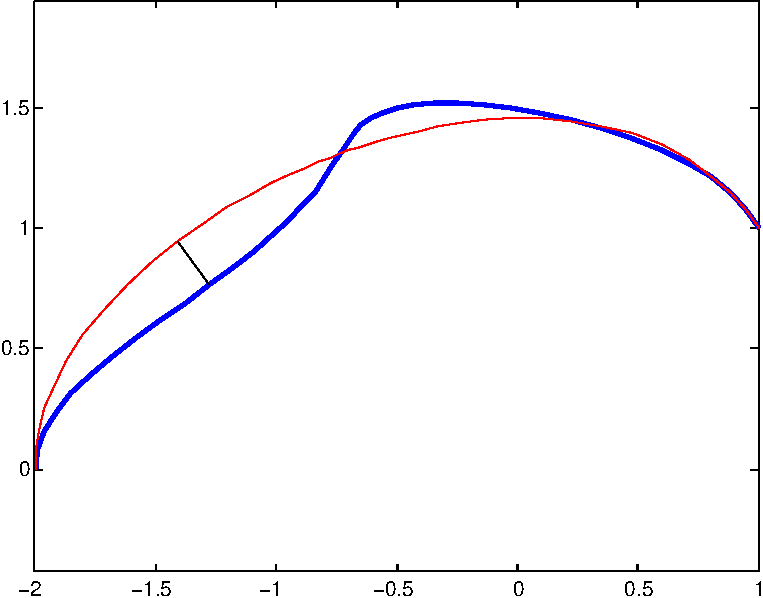
\includegraphics[scale=0.5]{kurvedeling1-crop.pdf}
    \caption{Before the split. The blue curve is the $\gamma$-curve, and the red curve is the Bezier curve. The black line corresponds to the $t$-value where the error between the curves is biggest.}
    \label{fig:kurvedeling1}
\end{minipage}\hfill
\begin{minipage}[t]{.45\textwidth}
\vspace{0pt}
    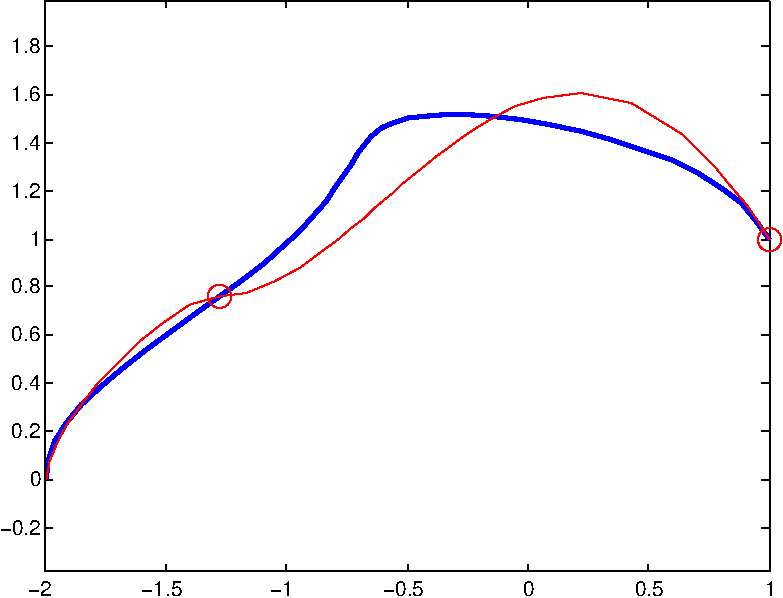
\includegraphics[scale=0.5]{kurvedeling2-crop.pdf}
    \caption{After the split. The blue curve us the $\gamma$-curve, and the red is the Bezier curve. The red circle is the end point of the new curves.}
    \label{fig:kurvedeling2}
\end{minipage}
\end{figure}


\subsection*{Unit tangent vectors}
The unit tangent vectors $\mathbf{v}_0$ and $\mathbf{v}_3$ can be found by using the data points $x$ and $y$ around the end points $\mathbf{P}_0$ and $\mathbf{P}_3$. We differ between tangent vectors from corners and tangent vectors that make the curve $C^1$.

A tangent vector that has its origin in a detected corner will only need data points from one side of the end point. The unit tangent vector is  $\mathbf{v}_i = \frac{[1, m_i]^T}{\sqrt{1+m_i^2}}$, where $m_i = (y_{i+r} - y_i)/(x_{i+r} - x_i)$ and $r$ is a positive integer denoting the number of data points away from the end point.

A tangent vector that has its origin in a new control point will need data points from both sides, since the curve should be $C^1$. The unit tangent vector is constructed in the same way as above, only with $m_i = (y_{i+r} - y_{i-r})/(x_{i+r} - x_{i-r})$.


\section*{Numerical experiments}

In this section we will present the results of our algorithm run on different test problems. We will see how smoothness in the corners affects the imaging, and we will see the effects of different values of the error tolerance. To be able to reconstruct the Bezier curves, we store the control points for each segment recursively.

If the error between a Bezier curve and the original curve is too large, the curve is divided in two in a new point $\mathbf{P}_i$ where the error is biggest. If $\mathbf{P}_i$ is closer to one of the endpoints than a certain space parameter, we choose to split the curve in the midpoint. After splitting, we construct a Bezier curve for each half, using the same method recursively. Let $U$ be a subset of points that generates a Bezier curve segment. If the splitting of $U$ results in subsets smaller than 3, splitting will not make a better approximation. To stop the recursion before it divides the curve too far, we included a space limitation in our algorithm. 

To obtain a curve that is $C^1$, the vector must be the tangent in $\mathbf{P}_i$ on the curve, with slope $m_i = (y_{i+r} - y_{i-r})/(x_{i+r} - x_{i-r})$. In the early stages of our research, we had some problems with the plotting of our Bezier curves; some parts of the curve were not drawn. The reason, we discovered, was that some of our matrices in the calculation of $\alpha_1$ and $\alpha_2$ were singular. This error arises when the tangent vectors, $\mathbf{v}_0$ and $\mathbf{v}_3$, are parallel. This happens either if $|U|$ is too small, or the denominator in $m_i$ is close to zero. To avoid the latter, we recommend $\mathbf{v}_i = [0,1]$ when $x_{i+r} - x_i$ is below some limit close to zero. One way of choosing $r$ is defining it as a fraction of the total number of data points, rounded upwards to the closest integer. We found that this generally gave better results for different shapes. Remark that $x_{i\pm r} \notin U$ for some $i,r \in \mathbb{N}$. To fix this, we simply choose a smaller $r'$  such that $x_{i\pm r'} \in U$.


We run our algorithm on the picture shown in Figure~\ref{fig:stitch} with corner detection and $tolerance = 2$. The result was 63 Bezier curves. The algorithm run without corner detection and tangent vectors making the shape $C^1$, gives 75 Bezier curves with the same conditions. Our image has many sharp edges, so it is clearly advantageous to detect the corners before constructing the Bezier curves. For a shape with smooth edges, the number of Bezier curves often goes slightly down when applying the algorithm without edge detection. This is especially when the tolerance for error is high. 

The Newton-Raphson iteration method has a great impact on our result. Because of fast convergence, we consider 10 iterations sufficient. Running the algorithm on the image in Figure~\ref{fig:stitch} without the method, results in 91 Bezier curves, an increase of 44 $\%$. Without corner detection, the result was 103 Bezier curves. 




\begin{figure}

\centering
\begin{minipage}[t]{.49\textwidth}
\centering
\vspace{0pt}
    
\includegraphics[scale=0.3]{disney.jpg}
\end{minipage}
\begin{minipage}[t]{.5\textwidth}
\centering
\vspace{0pt}
    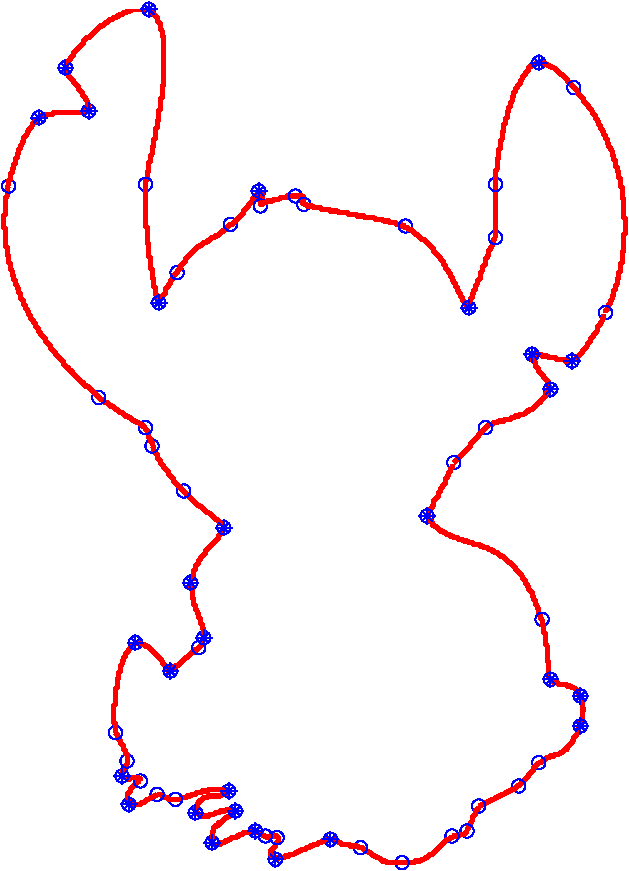
\includegraphics[scale=0.52]{figure6-crop.pdf}
\end{minipage}\hfill
\caption{The picture to the left shows the original image to be fitted. The picture to the right shows the approximated curve consisting of 63 Bezier curves. The starred points are detected corners before curve fitting. The circled dots illustrate the new end points where the Bezier curves are split in two. The picture is collected from \cite{pic:stitch}}
\label{fig:stitch}
\end{figure}

The tolerance is a unitless size which depends on the number of data points from the shape. Thus, small images need a lower tolerance to get a good approximation to the shape.  An illustration of this is shown in Figure~\ref{fig:mickey}. The algorithm is run on the same shape with $tolerance = 10$, but with different image size. The smaller set of data points constructs a less accurate fit to the original shape even though the original images look practically the same. 

\begin{figure}

\centering
\begin{minipage}[t]{.24\textwidth}
\centering
\vspace{0pt}
    
\includegraphics[scale=0.09]{mickey.jpg}
\end{minipage}
\begin{minipage}[t]{.24\textwidth}
\centering
\vspace{0pt}
    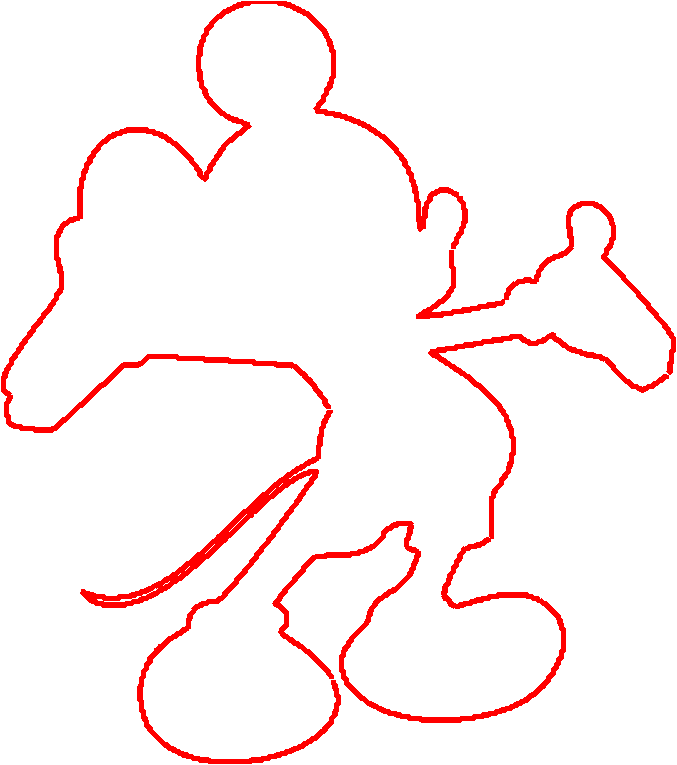
\includegraphics[scale=0.3]{mickey1-crop.pdf}
\end{minipage}\hfill
\begin{minipage}[t]{.24\textwidth}
\centering
\vspace{0pt}
    
\includegraphics[scale=0.3]{mickey2.jpg}
\end{minipage}
\begin{minipage}[t]{.24\textwidth}
\centering
\vspace{0pt}
    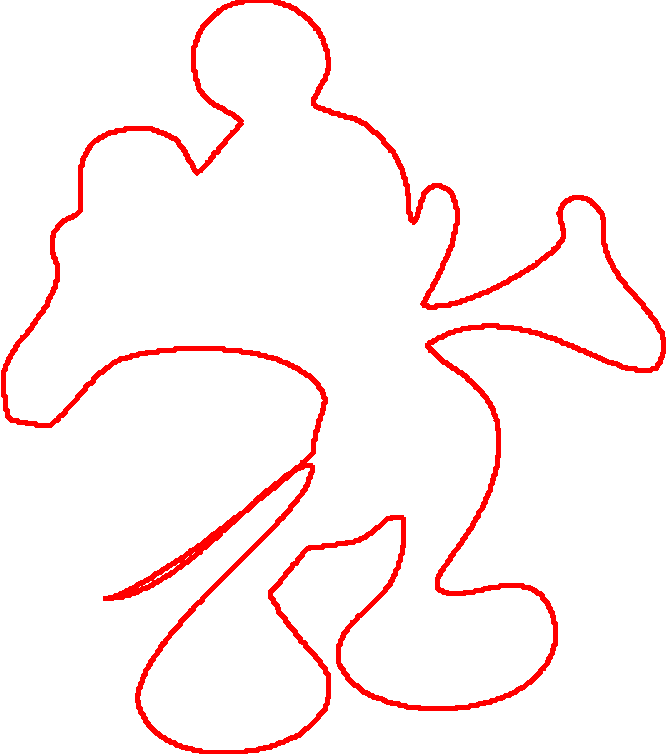
\includegraphics[scale=0.3]{mickey2-crop.pdf}
\end{minipage}\hfill
\caption{Curve fitting with same tolerance and different image sizes. The image to the left is of size 149 kB and constructs the approximated curve next to it. The image to rhe right is of size 99 kB and constructs a much less accurate curve with the same tolerance. The pictures are collected from \cite{pic:mickey1} and \cite{pic:mickey2}.}
\label{fig:mickey}
\end{figure}





\section*{Conclusion}
In this paper we have fitted cubic Bezier curves to shapes of choice.

We were able to minimize the number of curves used for a given error tolerance by using the Newton-Raphson method for finding optimal $t$-values. If the error isn't small enough after a given number of iterations, the curve is divided in two. Problems occured when horizontal lines were to be approximated. This was fixed by adding a default tangent vector, and a limitation for the dividing of curves. With our algorithm it is also possible to display the number of curves used, and the points that are used to generate the Bezier curves.



\bibliographystyle{plain}
\bibliography{bezierbib}   % Insert you own BibTeX file 


\end{document}  
